\documentclass[11pt,a4paper]{article}
\usepackage{../ma362}
\usepackage{tikz}
\usetikzlibrary{decorations.markings}
\usetikzlibrary{math,calc,arrows.meta}

\semester{Fall}
\year{2019}
\subtitlenumber{11}
\author{刘逸灏 (515370910207)}
\newcommand{\res}[1]{\mathop{\Res}\limits_{#1}}

\begin{document}
\maketitle

\section{六(一)/6}
\begin{problem}
仿照例6.15的方法计算下列积分:
\begin{enumerate}
  \item $\displaystyle\int_0^{+\infty}\frac{\sin x}{x(x^2+a^2)}dx\quad(a>0)$;
  \item $\displaystyle\int_0^{+\infty}\frac{\sin x}{x(x^2+1)^2}dx$.
\end{enumerate}
\end{problem}
\subsection*{(1)}
被积函数是偶函数, 故
$$\int_0^{+\infty}\frac{\sin x}{x(x^2+a^2)}dx=\frac{1}{2}\text{P.V.}\int_{-\infty}^{+\infty}\frac{\sin x}{x(x^2+a^2)}dx,$$
$$f(z)=\frac{e^{iz}}{z(z^2+a^2)}=\frac{e^{iz}}{z(z-ia)(z+ia)}.$$
$0$为一阶极点, $ia$为一阶极点, $-ia$为一阶极点, 只有$ia$在上半平面内.
$$\res{z=ia}=\left.\frac{e^{iz}}{z(z+ia)}\right|_{z=ia}=-\frac{e^{-a}}{2a^2}.$$
考虑$f(z)$在上半平面内沿下图所示之闭曲线路径$C$的积分.
\begin{center}
  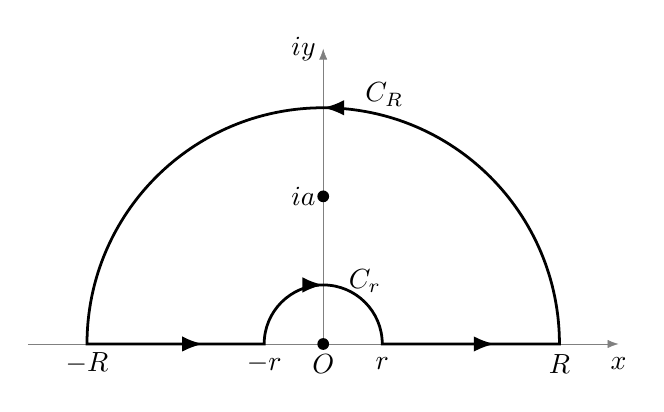
\begin{tikzpicture}[>/.tip={Latex}]
    % The axes
    \tikzmath{\r=0.75;\R=3;\a=0.5*\r+0.5*\R;}
    \draw[help lines,->] (-1.25*\R,0) -- (1.25*\R,0) coordinate (xaxis);
    \draw[help lines,->] (0,0) -- (0,1.25*\R) coordinate (yaxis);
    % The integral path
    \draw[
      line width=1pt,
      decoration={
          markings,
          mark=at position 0 with {\arrow{>}},
          mark=at position 0.16 with {\arrow{>}},
          mark=at position 0.5 with {\arrow{>}},
          mark=at position 0.88 with {\arrow{>}},
        },
      postaction={decorate}
    ] (0,\r) arc(90:0:\r) -- (\r,0)
    -- (\R,0) arc(0:180:\R) -- (-\R,0)
    -- (-\r,0) arc(180:90:\r) -- cycle;

    \node at (-\r,-0.25) {$-r$};
    \node at (\r,-0.25) {$r$};
    \node at (-\R,-0.25) {$-R$};
    \node at (\R,-0.25) {$R$};
    \node at (0,-0.25) {$O$};
    \node[circle,fill,inner sep=1.5pt] at (0,0) {};
    \node at (-0.25,\a) {$ia$};
    \node[circle,fill,inner sep=1.5pt] at (0,\a) {};
    \node at (1.25*\R,-0.25) {$x$};
    \node at (-0.25,1.25*\R) {$iy$};
    \node[above] at (45:\r) {$C_r$};
    \node[above] at (75:\R) {$C_R$};
  \end{tikzpicture}
\end{center}
由留数定理得
$$\int_r^Rf(x)dx+\int_{C_R}f(z)dz+\int_{-R}^{-r}f(x)dx-\int_{C_r}f(z)dz=2\pi i\res{z=ia}=2\pi i\cdot -\frac{e^{-a}}{2a^2}=-i\pi\frac{e^{-a}}{a^2}.$$
由引理6.2知
$$\lim_{R\to+\infty}\int_{C_R}f(z)dz=\lim_{R\to+\infty}\int_{C_R}\frac{e^{iz}}{z(z^2+a^2)}dz=0.$$
由引理6.3知
$$\lim_{r\to0}\int_{C_r}f(z)dz=\lim_{r\to0}\int_{C_r}\frac{e^{iz}}{z(z^2+a^2)}dz=i\pi\lim_{r\to0}\frac{e^{iz}}{z^2+a^2}=i\pi\frac{1}{a^2}.$$
另$r\to0$, $R\to+\infty$可得
$$\text{P.V.}\int_{-\infty}^{+\infty}\frac{e^{ix}}{x(x^2+a^2)}dx=i\pi\frac{1-e^{-a}}{a^2}.$$
且
$$\int_{-\infty}^{+\infty}\frac{e^{ix}}{x(x^2+a^2)}dx=\int_{-\infty}^{+\infty}\frac{\cos x}{x(x^2+a^2)}dx+i\int_{-\infty}^{+\infty}\frac{\sin x}{x(x^2+a^2)}dx.$$
故
$$\int_0^{+\infty}\frac{\sin x}{x(x^2+a^2)}dx=\frac{\pi(1-e^{-a})}{2a^2}.$$
\subsection*{(2)}
被积函数是偶函数, 故
$$\int_0^{+\infty}\frac{\sin x}{x(x^2+1)^2}dx=\frac{1}{2}\text{P.V.}\int_{-\infty}^{+\infty}\frac{\sin x}{x(x^2+1)^2}dx,$$
$$f(z)=\frac{e^{iz}}{z(z^2+1)^2}=\frac{e^{iz}}{z(z-i)^2(z+i)^2}.$$
$0$为一阶极点, $i$为二阶极点, $-i$为二阶极点, 只有$i$在上半平面内.
$$\res{z=i}=\left.\left[\frac{e^{iz}}{z(z+i)^2}\right]'\right|_{z=i}=\left.\frac{ie^{iz}(z^2+4iz-1)}{z^2(z+i)^3}\right|_{z=i}=-\frac{3}{4e}.$$
考虑$f(z)$在上半平面内沿下图所示之闭曲线路径$C$的积分.
\begin{center}
  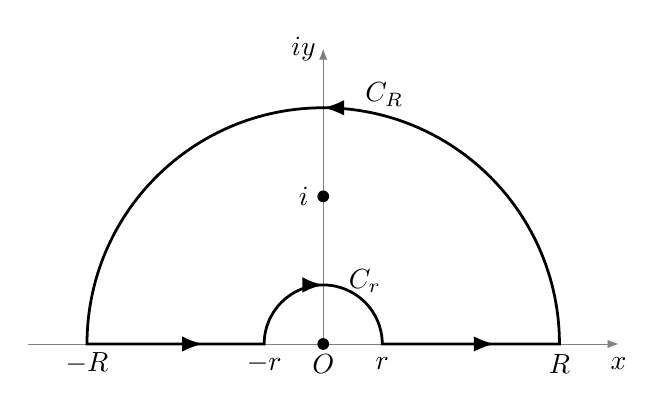
\begin{tikzpicture}[>/.tip={Latex}]
    % The axes
    \tikzmath{\r=0.75;\R=3;\a=0.5*\r+0.5*\R;}
    \draw[help lines,->] (-1.25*\R,0) -- (1.25*\R,0) coordinate (xaxis);
    \draw[help lines,->] (0,0) -- (0,1.25*\R) coordinate (yaxis);
    % The integral path
    \draw[
      line width=1pt,
      decoration={
          markings,
          mark=at position 0 with {\arrow{>}},
          mark=at position 0.16 with {\arrow{>}},
          mark=at position 0.5 with {\arrow{>}},
          mark=at position 0.88 with {\arrow{>}},
        },
      postaction={decorate}
    ] (0,\r) arc(90:0:\r) -- (\r,0)
    -- (\R,0) arc(0:180:\R) -- (-\R,0)
    -- (-\r,0) arc(180:90:\r) -- cycle;

    \node at (-\r,-0.25) {$-r$};
    \node at (\r,-0.25) {$r$};
    \node at (-\R,-0.25) {$-R$};
    \node at (\R,-0.25) {$R$};
    \node at (0,-0.25) {$O$};
    \node[circle,fill,inner sep=1.5pt] at (0,0) {};
    \node at (-0.25,\a) {$i$};
    \node[circle,fill,inner sep=1.5pt] at (0,\a) {};
    \node at (1.25*\R,-0.25) {$x$};
    \node at (-0.25,1.25*\R) {$iy$};
    \node[above] at (45:\r) {$C_r$};
    \node[above] at (75:\R) {$C_R$};
  \end{tikzpicture}
\end{center}
由留数定理得
$$\int_r^Rf(x)dx+\int_{C_R}f(z)dz+\int_{-R}^{-r}f(x)dx-\int_{C_r}f(z)dz=2\pi i\res{z=ia}=2\pi i\cdot -\frac{3}{4e}=-i\pi\frac{3}{2e}.$$
由引理6.2知
$$\lim_{R\to+\infty}\int_{C_R}f(z)dz=\lim_{R\to+\infty}\int_{C_R}\frac{e^{iz}}{z(z^2+1)^2}dz=0.$$
由引理6.3知
$$\lim_{r\to0}\int_{C_r}f(z)dz=\lim_{r\to0}\int_{C_r}\frac{e^{iz}}{z(z^2+1)^2}dz=i\pi\lim_{r\to0}\frac{e^{iz}}{(z^2+1)^2}=i\pi.$$
另$r\to0$, $R\to+\infty$可得
$$\text{P.V.}\int_{-\infty}^{+\infty}\frac{e^{ix}}{x(x^2+1)^2}dx=i\pi\left(1-\frac{3}{2e}\right).$$
且
$$\int_{-\infty}^{+\infty}\frac{e^{ix}}{x(x^2+1)^2}dx=\int_{-\infty}^{+\infty}\frac{\cos x}{x(x^2+1)^2}dx+i\int_{-\infty}^{+\infty}\frac{\sin x}{x(x^2+1)^2}dx.$$
故
$$\int_0^{+\infty}\frac{\sin x}{x(x^2+1)^2}dx=\pi\left(\frac{1}{2}-\frac{3}{4e}\right).$$

\section{六(一)/10}
\begin{problem}
证明方程
$$e^{z-\lambda}=z\quad(\lambda>1)$$
在单位圆$|z|<1$内恰有一个根, 且为实根.
\end{problem}
设$f(z)=z$, $\varphi(z)=-e^{z-\lambda}$, $C$是单位圆$|z|=1$, 则$f(z)$和$\varphi(z)$在$C$内部均解析, 且在$C$上
$$|f(z)|=|z|=1>|e^{z-\lambda}|=|\varphi(z)|.$$
根据儒歇定理可知$f(z)$和$f(z)+\varphi(z)=z-e^{z-\lambda}$在$C$内有同样多的零点. 显然$f(z)$在$C$内只有一个零点$z=0$, 故方程
$e^{z-\lambda}=z$在$C$内也只有一个零点. 作实连续函数
$$g(z)=z-e^{z-\lambda},$$
$$g(-1)=-1-e^{-1-\lambda}<0,\quad g(1)=1-e^{1-\lambda}>0.$$
根据零点定理可得$g(z)$在$(-1,1)$有一个实零点, 故得证.

\section{六(一)/11}
\begin{problem}
证明方程
$$e^z-e^\lambda z^n=0\quad(\lambda>1)$$
在单位圆$|z|<1$内有$n$个根.
\end{problem}
设$f(z)=e^\lambda z^n$, $\varphi(z)=-e^z$, $C$是单位圆$|z|=1$, 则$f(z)$和$\varphi(z)$在$C$内部均解析, 且在$C$上
$$|f(z)|=\left|e^{\lambda+n(\ln z+2k\pi i)}\right|=|e^{\lambda+n\ln z}|=|e^\lambda|>|e^z|=|\varphi(z)|.$$
根据儒歇定理可知$f(z)$和$f(z)+\varphi(z)=e^\lambda z^n-e^z$在$C$内有同样多的零点. 根据代数学基本定理可知$n$维多项式$f(z)$有$n$个零点, 故方程有$n$个根.

\section{六(一)/12}
\begin{problem}
若$f(z)$在周线$C$内部除有一个一阶极点外解析, 且连续到$C$, 在$C$上$|f(z)|=1$. 证明
$$f(z)=a\quad(|a|>1)$$
在$C$内部恰好有一个根.
\end{problem}
$$P(f(z)-a,C)=P(f(z),C)=1.$$
要证明$N(f(z)-a,C)=1$, 只需证明
$$N(f(z)-a,C)-P(f(z)-a,C)=\frac{\Delta_C\arg(f(z)-a)}{2\pi}=0,$$
作$\eta=f(z)-a$, 将$z$平面上的周线$C$变换为$\eta$平面上的闭曲线$\Gamma$. 由于$|f(z)|=1$, $\Gamma$全在圆周$|\eta+a|=1$的内部. 又因为$|a|>1$可知原点$\eta=0$不在该圆周内部, 点$\eta$不会围着$\eta=0$绕行, 故
$$\Delta_C\arg(f(z)-a)=0.$$
即$f(z)=a$在$C$内部恰好有一个根.

\section{六(一)/13}
若$f(z)$在周线$C$内部亚纯且连续到$C$, 试证
\begin{enumerate}
  \item 若$z\in C$时, $|f(z)|<1$, 则方程$f(z)=1$在$C$内部根的个数, 等于$f(z)$在$C$内部的极点个数.
  \item 若$z\in C$时, $|f(z)|>1$, 则方程$f(z)=1$在$C$内部根的个数, 等于$f(z)$在$C$内部的零点个数.
\end{enumerate}

\subsection*{(1)}
$$P(f(z)-1,C)=P(f(z),C).$$
要证明$N(f(z)-1,C)=P(f(z),C)$, 只需证明
$$N(f(z)-1,C)-P(f(z)-1,C)=\frac{\Delta_C\arg(f(z)-1)}{2\pi}=0,$$
作$\eta=f(z)-1$, 将$z$平面上的周线$C$变换为$\eta$平面上的闭曲线$\Gamma$. 由于$|f(z)|<1$, $\Gamma$全在圆周$|\eta+1|=1$的内部. 原点$\eta=0$不在该圆周内部, 点$\eta$不会围着$\eta=0$绕行, 故
$$\Delta_C\arg(f(z)-1)=0.$$
即方程$f(z)=1$在$C$内部根的个数, 等于$f(z)$在$C$内部的极点个数.

\subsection*{(2)}
作$g(z)=\dfrac{1}{f(z)}$, 则$|g(z)|<1$. 根据(1)可得方程$g(z)=1$在$C$内部根的个数, 等于$g(z)$在$C$内部的极点个数. 由于$g(z)=1$时, $f(z)=1$, 且$g(z)$的极点就是$f(z)$的零点, 故方程$f(z)=1$在$C$内部根的个数, 等于$f(z)$在$C$内部的零点个数.

\section{六(一)/14}
\begin{problem}
设$\varphi(z)$在$C:|z|=1$内部解析, 且连续到$C$, 在$C$上$|\varphi(z)|<1$. 试证: 在$C$内部只有一个点$z_0$, 使$\varphi(z_0)=z_0$.
\end{problem}

设$f(z)=z$, 则$f(z)$在$C$内部均解析, 且在$C$上
$$|f(z)|=|z|=1>|-\varphi(z)|.$$
根据儒歇定理可知$f(z)$和$f(z)-\varphi(z)=z-\varphi(z)$在$C$内有同样多的零点. 显然$f(z)$在$C$内只有一个零点$z=0$, 故方程
$\varphi(z)=z$在$C$内也只有一个零点. 即在$C$内部只有一个点$z_0$, 使$\varphi(z_0)=z_0$.

\end{document}
